\chapter{Service and Maintenance}
\thispagestyle{fancy}
\minitoc[n] % Creating an actual minitoc

\section{General}
This section provides information on handling, service and maintenance of the aircraft.

The owner can obtain up-to-date service bulletins from the Van’s web site at www.vansaircraft.com. 
Service bulletins on the Lycoming Kit engine can be obtained from www.lycoming.com and any information relating to the installed propeller from the Hartzell
manufacturer at www.hartzellprop.com.

The South African CAA or the Aero Club of South Africa may also issue information and directives. These
directives could be advisory or mandatory. As failure to implement such a directive could contravene the
issued Permit to Fly (as well as risking safety) It is essential the owner keep up to date on all such
relevant information relating to the aircraft, and its installed systems equipment.

\section{Ground Handling}
Ground towing/non-taxi movement can be accomplished by manoeuvring with the castoring tail wheel.  When
taxiing the aircraft ensure that the taxi path and propeller back blast areas are clear. In the first few feet of taxi
apply the brakes to ensure effectiveness. Do not operate the engine at high rpm, taxi with care
When parking, ensure aircraft is  protected from adverse weather and that it presents no danger to
others. Park the aircraft into wind if possible and tie down securely.


\section{Maintenance and Service}
Refer to the Reference section for 50/100hr/annual maintenance requirements and overhaul time periods.

All work should be entered in the appropriate log book indicating:-
\begin{itemize}
  \item Date work was done
  \item Description of work 
  \item Number of hours recorded on the aircraft at that time.
  \item Name and signature of individual doing the work.
\end{itemize}

\subsection{25 Hour Inspection}
The following 25-hour check is in essence a detailed pre-flight developed from relevant sources and based on best practice. 

\subsubsection{Engine compartment}
Remove engine cowls for general inspection including the following: 
\begin{enumerate}
\item Oil hoses and filter. Check for leaks and security.
\item Oil cooler. General check of installation
\item Oil. Check level and review top up frequency
\item Induction filter. Check filter visually
\item Fuel injection servo/Carburettor. General exterior check including control cables.
\item Magneto. General exterior inspection and security
\item Plug leads. Inspect for condition
\item Fuel hoses. Check for leaks and signs of loosening
\item Fuel pump. Check body joins for leaks
\item Exhaust system. Check for blowing manifold gaskets
\item Check heat muffs and ducting
\item Check joints for wear/damage. Check mounting points
\item Check general integrity of system
\item Engine mount. Check for damage
\item Brake fluid. Check level, note change since last service.
\item Compartment wiring. Check for damage and security.
\item Cooling system. Check for damage/wear/security.
\item Check baffles and flexible sealing strips.
\item General. Review/inspection of engine compartment
\item Cowls. Inspect for damage.
\item Replace cowls
\end{enumerate}
\subsubsection{Propeller inspection}
\begin{enumerate}
\item Propeller. Check for nicks, scratches, leaks or corrosion.
\item Spinner. Check spinner and back plate for condition.
\end{enumerate}
\subsubsection{External inspection}
\begin{enumerate}
\item Remove all wheel spats:
\item Tyres. Check pressures, mains  30-35 psi. (Cold) %and nose
\item Inspect tyres for wear and slip on hub.
\item Brake system. Inspect brake pads, replace if appropriate.
\item Inspect hydraulic lines, joints and bleed points.
\item Wheels. Check bearings for play. Check split pins and bolts for security, including the split-hub bolts.
\item Spats. Inspect for damage, replace wheel spats.
\item General airframe and control surfaces review including, but not limited to:
\item Control surfaces. Individual inspection of each surface for free movement, satisfactory mounting/hinge condition
and actuating system integrity, particular attention should be given to flap actuating rods as the rod end is not
safe tied.
\item Fibreglass components. General inspection for integrity.
\item Fuel tanks. Inspect for leaks and security.
\end{enumerate}


\section{Propeller Maintenance}
\subsection{Lubrication Intervals}
\begin{enumerate}
\item 
The propeller must be lubricated at intervals not to 
exceed 100 hours or at 12 calendar months, whichever 
occurs first.
\subitem
If annual operation is significantly less than 100 
hours, calendar lubrication intervals should be 
reduced to six months.
\subitem
If the aircraft is operated or stored under adverse 
atmospheric conditions, e.g., high humidity, salt air, 
calendar lubrication intervals should be reduced to 
six months.
\item
Owners of high use aircraft may wish to extend their 
lubrication interval. Lubrication interval may be gradually 
extended after evaluation of previous propeller overhauls 
with regard to bearing wear and internal corrosion.
\item 
Hartzell Propeller Inc. recommends that new or newly 
overhauled propellers be lubricated after the first one or 
two hours of operation because centrifugal loads will pack 
and redistribute grease, which may result in a propeller 
imbalance. Redistribution of grease may also result in 
voids in the blade bearing area where moisture can collect.
\end{enumerate}

\section{Battery Maintenance}
The State of Charge of the battery can be determined from Figure~\ref{fig:SOC}.

\begin{figure}[H]
\centering
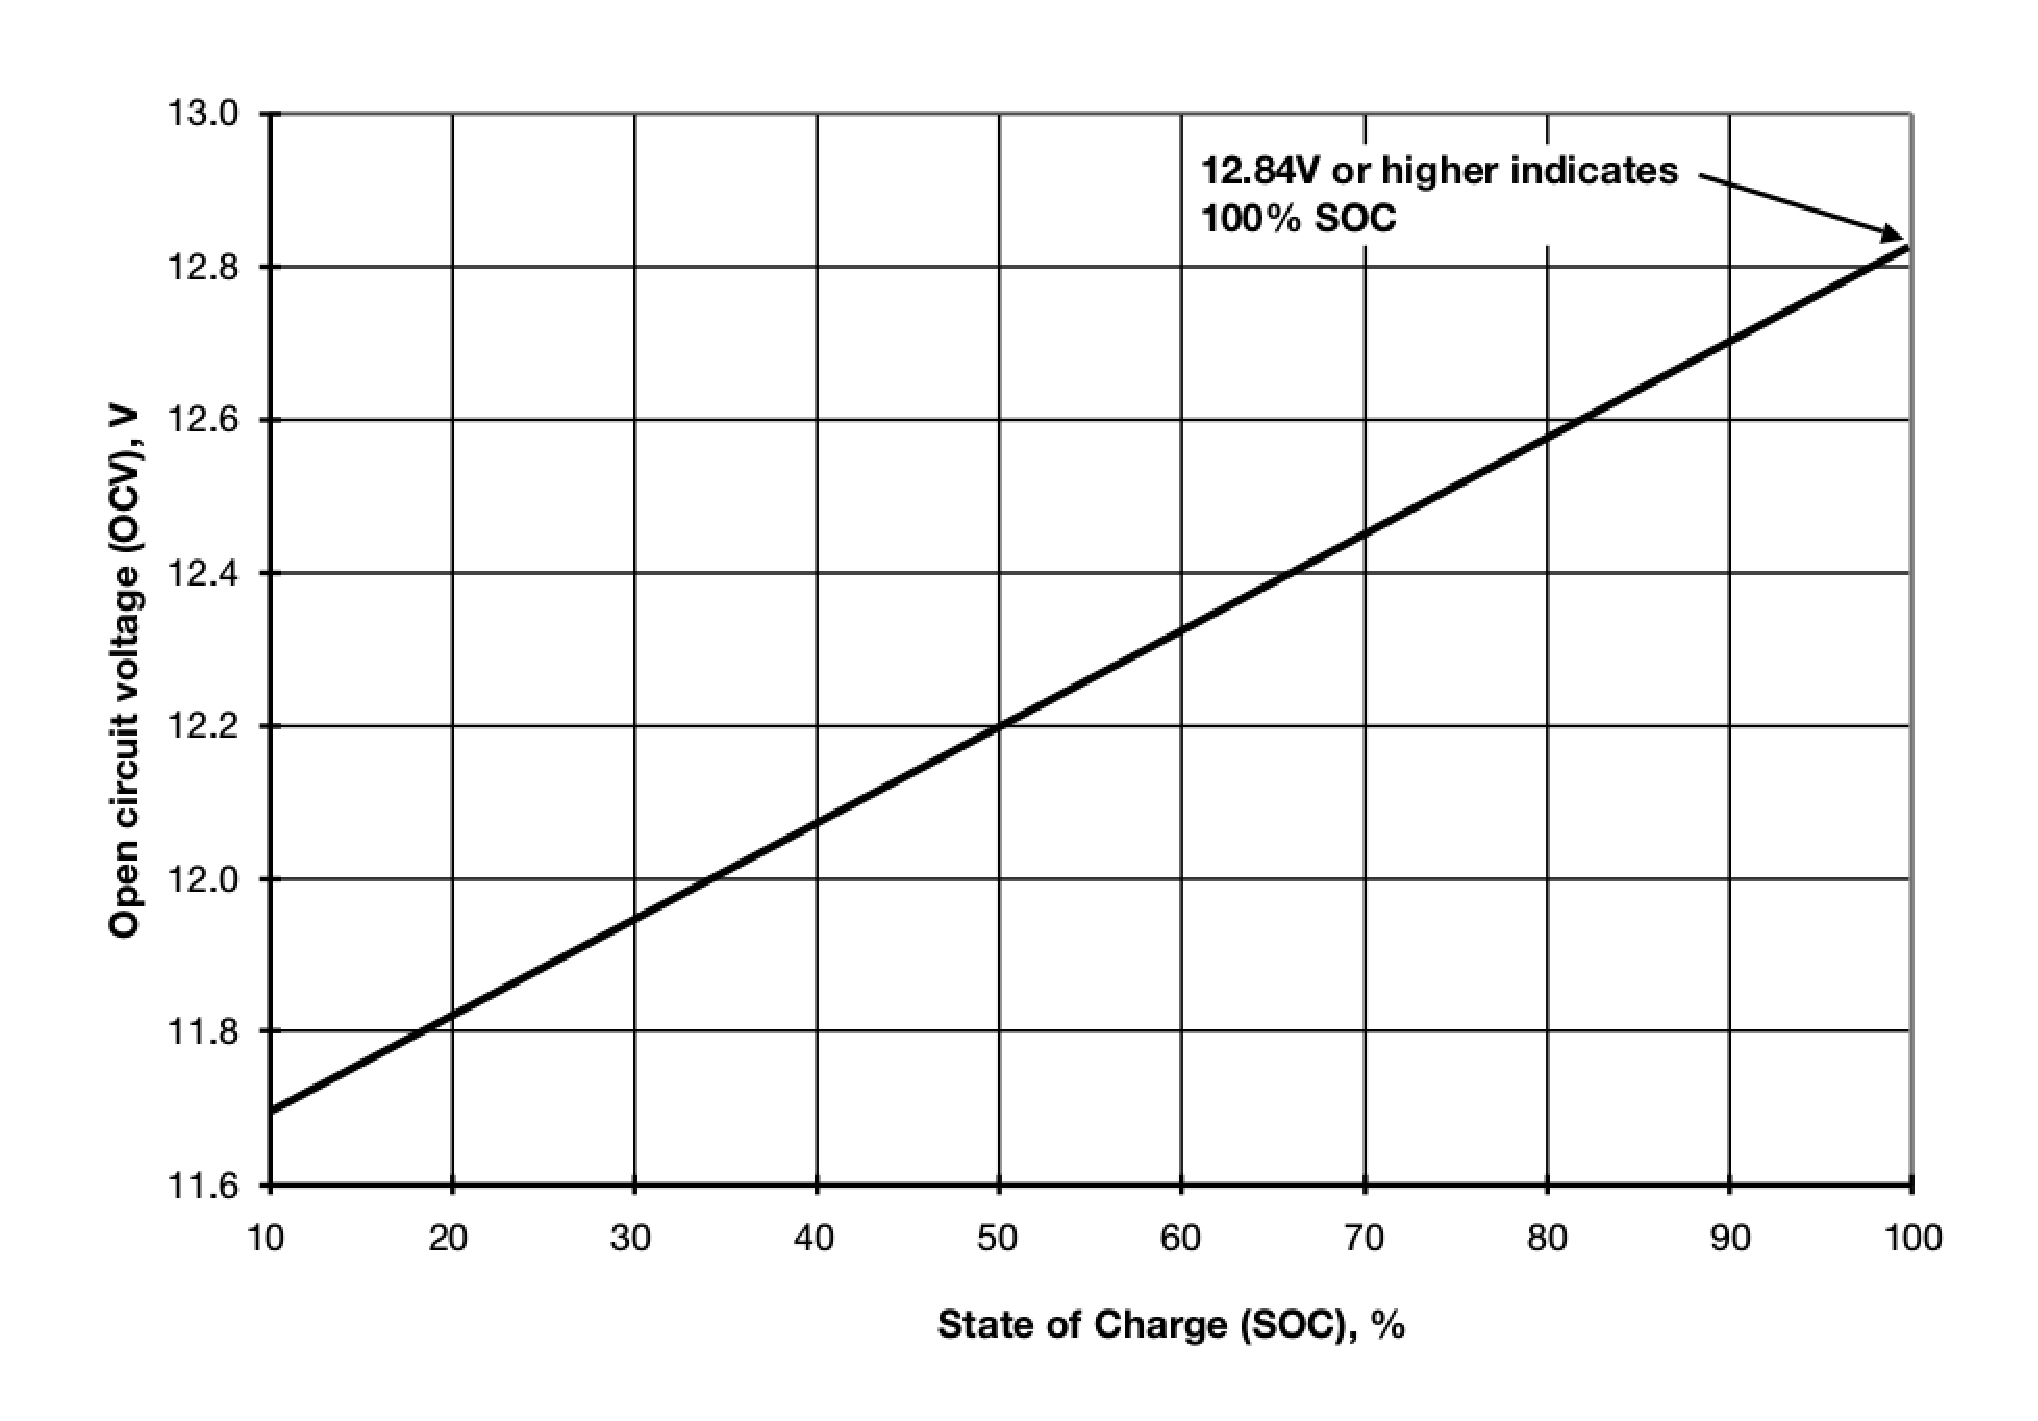
\includegraphics[height=0.7\textwidth]{stateofcharge.eps}
\caption{State of Charge}
\label{fig:SOC}
\end{figure}

To get long life from the battery, it is important that the battery is kept near full charge, approximately 12.8V.  If there are electrical loads during storage, then the negative battery cable should be disconnected OR an independent float charger used.
